\documentclass[a4paper,12pt]{article}

\usepackage{a4wide}
\usepackage{amsfonts}
\usepackage{amsmath}
\usepackage{amssymb}
\usepackage{lipsum}
\usepackage{float}
\usepackage{graphicx}  % For including images

\usepackage{xcolor}  % For a colorfull presentation
\usepackage{listings}  % For presenting code 

\usepackage{hyperref}
\usepackage{xcolor}
\usepackage{listings}

\definecolor{mGreen}{rgb}{0,0.6,0}
\definecolor{mGray}{rgb}{0.5,0.5,0.5}
\definecolor{mPurple}{rgb}{0.58,0,0.82}
\definecolor{backgroundColour}{rgb}{0.95,0.95,0.92}
%TODO:Figure out how to make a nice style
\lstdefinestyle{mystyle}{
  language=Python,
  basicstyle=\ttfamily\footnotesize,
  backgroundcolor=\color[HTML]{F7F7F7},
  rulecolor=\color[HTML]{EEEEEE},
  identifierstyle=\color[HTML]{24292E},
  emphstyle=\color[HTML]{005CC5},
  keywordstyle=\color[HTML]{D73A49},
  commentstyle=\color[HTML]{6A737D},
  stringstyle=\color[HTML]{032F62},
  emph={@property,self,range,True,False},
  morekeywords={super,with,as,lambda},
  literate=%
    {+}{{{\color[HTML]{D73A49}+}}}1
    {-}{{{\color[HTML]{D73A49}-}}}1
    {*}{{{\color[HTML]{D73A49}*}}}1
    {/}{{{\color[HTML]{D73A49}/}}}1
    {=}{{{\color[HTML]{D73A49}=}}}1
    {/=}{{{\color[HTML]{D73A49}=}}}1,
  breakatwhitespace=false,
  breaklines=true,
  captionpos=b,
  keepspaces=true,
  numbers=none,
  showspaces=false,
  showstringspaces=false,
  showtabs=false,
  tabsize=4,
  frame=single,
}
% Definition of a style for code, matter of taste
\lstset{style=mystyle}

%Custom commands
%\renewcommand{\thesection}{Task \arabic{section}}
\newcommand{\ispc}{\textmd{ispc}}

\begin{document}
\title{Assignment 3}
\author{Sophus Valentin Willumsgaard hwx333}
\date{11/12/2024}
\maketitle

% Please leave the table of contents as is, for the ease of navigation for TAs
All the programs have been benchmarked on hendrixfut01fl
\section*{Task 1:
  Flattening with the New, More Efficient Rules}
I will here show the sections that differ from classicKer.

flags1 is defined with integers values. I ended up using sized to declare it
has the same length. the same flags as in classicKer is then defined from
flags1.
\begin{lstlisting}
  -- make offsets and flag array
  let (Ba, flags1) = mkFlagArray Sa 0 (iota m)
  let Ba = map (i64.u32) Ba
  let flags1 = sized n flags1
  let flags = map (bool.i64) flags1
\end{lstlisting}
We define the inner and outer segments as in the lecture slides
\begin{lstlisting}
  let II1a = sgmScan (+) 0 flags flags1
  let II2a = map2 (\i sgm -> i - Ba[sgm]) (iota n) II1a
\end{lstlisting}
The replicate and iota transforms are then replaced with optimized
transformation as in slides
\begin{lstlisting}
  -- replicate bofinds inside map
  let rep_b = gather bofinds II1a
  -- replicate cs inside map
  let rep_c = gather cs II1a
  -- iota inside map
  let iotis = II2a
\end{lstlisting}
The whole code is here
\begin{lstlisting}
def optimII1Ker [m][n][q] (Sa: [m]u32, Da: [n]f32)
                          (Sb: [m]u32, Db: [q]f32)
                          (cs: [m]f32) (inds: [m]i64)
                        : [m]f32 = #[unsafe]
  -- Task 1: please replace the dummy implementation below
  --         with a correct and efficient one

  -- make offsets and flag array
  let (Ba, flags1) = mkFlagArray Sa 0 (iota m)
  let Ba = map (i64.u32) Ba
  let flags1 = sized n flags1
  let flags = map (bool.i64) flags1
  --
  let (Bb, _) = mkFlagArray Sb false (replicate m true)
  let II1a = sgmScan (+) 0 flags flags1
  let II2a = map2 (\i sgm -> i - Ba[sgm]) (iota n) II1a
  -- replicate bofinds inside map
  let bofinds = map2 (\off ind -> Db[i64.u32 off+ind]) Bb inds
  let rep_b = gather bofinds II1a
  -- replicate cs inside map
  let rep_c = gather cs II1a
  -- map inside map
  let tmp1s = map3 (\ a b c -> (f32.sqrt a) * b + c) Da rep_b rep_c
  -- iota inside map
  let iotis = II2a
  -- map inside map
  let iotfs = map f32.i64 iotis
  -- map inside map
  let tmp2s = map2 (+) tmp1s iotfs
  -- reduce inside map
  let res =
    let tmp_scan = sgmScan f32.max f32.lowest flags tmp2s
    in  imap2 (iota m) Sa
          (\i s -> if s <= 0 then f32.lowest
                   else if i == m-1
                        then tmp_scan[n-1]
                        else tmp_scan[Ba[i+1]-1]
          )
  in  res
\end{lstlisting}
This code passes the validation tests, given in the assignment.
\section*{Task 2: Flattening Rule for Scatter inside Map }
let dx be the values of xss, and so for di and dv.
Furthermore let b1x be the offsets for xss (the offset defined with
exclusive scan), and II1i be segment indices.
\begin{lstlisting}
-- We first finde the values of the indices in the flattened array,
-- by adding the offsets of the array they are in.
let tmp = gather b1x II1i
let new_di = map2 (+) tmp di
-- we now just apply scatter to the total array.
in scatter dx new_di vss
\end{lstlisting}
\section*{Task 3: Flattening Rule for Histogram inside Map}
This is very similar to the previous exercise
let dhist be the values of histos, and so for di and dv.
Furthermore let b1hist be the offsets for histos, and II1i be segment indices.
\begin{lstlisting}
-- We first finde the values of the indices in the flattened array,
-- by adding the offsets of the array they are in.
let tmp = gather b1hist II1i
let new_di = map2 (+) tmp di
-- we now just apply reduce_by_index to the total array.
in reduce_by_index (o) (0_o) dhist new_di dv
\end{lstlisting}
%TODO: Google the notation here
\section*{Task 4: Implement the lifted version of \textmd{partition2}}
We have the following implementation of quicksort.
\begin{lstlisting}
def gather 'a (xs: []a) (is: []i32) =
  map (\i -> xs[i]) is
let partition2L 't [n] [m]
                -- the shape of condsL is also shp
                (condsL: [n]bool) (dummy: t)
                (shp: [m]i32, arr: [n]t) :
                ([m]i32, ([m]i32, [n]t)) =
  -- Here we have all auxiliary data
  let begs   = map2 (-) (scan (+) 0 shp) shp
  let flags  = mkFlagArray shp 0i32 (map (+1) (map i32.i64 (iota m)))
  let flags = sized n flags
  let outinds= sgmSumInt flags <| map (\f -> if f==0 then 0 else f-1) flags

  -- maps are lifted just to maps 
  let tflgs = map (\ c -> if c then 1 else 0) condsL
  let fflgs = map (\ b -> 1 - b) tflgs
  -- scan are lifted to segmented scan.
  let indsT = sgmSumInt flags tflgs
  let tmp   = sgmSumInt flags fflgs
  -- the single if statement are listed to a map.
  -- Note that outsets are added so we hit the right index.
  let lst   = map2 (\n sgm -> if n > 0 then indsT[sgm + n-1] else -1i32) shp begs
  -- the addition of lst instead becomes array addition of the corresponding lst values.
  let indsF = map2 (+) tmp (gather lst outinds)
  -- the map3 just becomes the same map3 on the flattened array.
  let inds  = map3 (\ c indT indF -> if c then indT-1i32 else indF-1) condsL indsT indsF
  -- We apply our scatter transformation
  let tmp1 = gather begs outinds
  let new_inds = map2 (+) tmp1 inds
  let fltarr= scatter (replicate n dummy) (map i64.i32 new_inds) arr
  in  (lst, (shp,fltarr))
\end{lstlisting}
in the comments in the code, I describe the different rules used to lift the
function.

The code validates the test given in assignment. I have then added a
further benchmark with random arrays of sizes increasing by a factor 10,
from 100 to 10000000, which gives the following results
\begin{figure}[htb!]
  \centering
  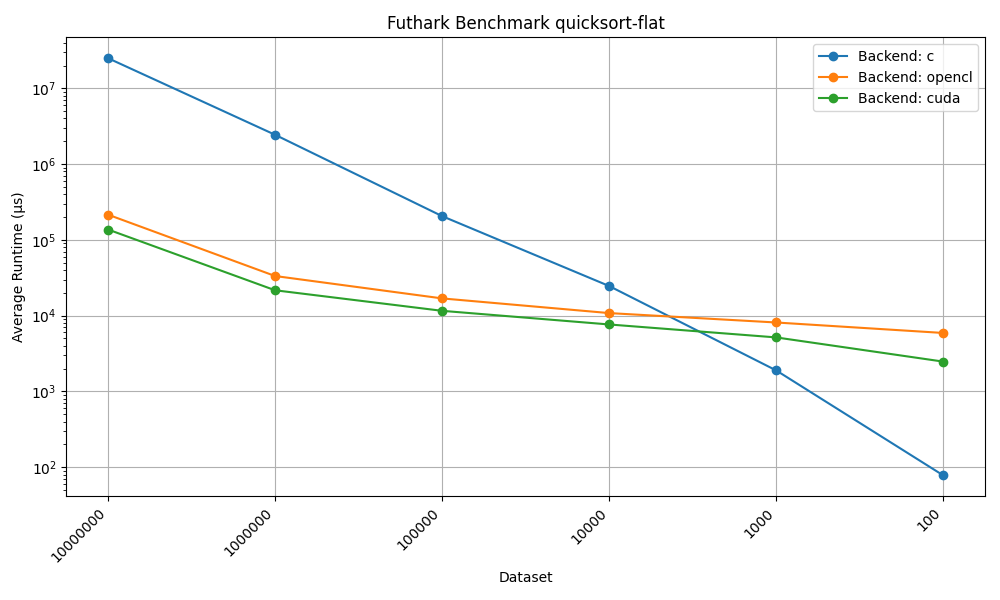
\includegraphics[width=\linewidth]{quicksort-flatbenchmark_results.png}
\end{figure}
We see that the sequential implementation looks to be close to \(O(n)\)
maybe \(O(\log n)\) which matches our expectation.
On the other hand the parallel opencl implementation, seems from 100 to
100000 seems to be performing like \(O(\log n)\) as there are only small
       increases in runtime, matching our expectation
\end{document}
